\section{Application and Measurement}
\label{sec:application}
\label{sec:measurement}

\subsection{Experimental Design}

We evaluate the framework on all 164 HumanEval+ tasks.  Before any model run,
we partition tasks into three equally sized modes using reference-solution
length, with cutoffs at 35 and 58 tokens.  The mode labels are used to fit and
evaluate posteriors but are not supplied as deployment labels.  We pair the
modes with three strategy-specific harnesses: a direct implementation prompt,
a structured specification-and-invariants prompt, and a robust decomposition
and edge-case prompt.

We execute Qwen2.5-Coder 1.5B, 7B, and 32B with each strategy for twenty
independent sampling attempts per task.  This gives
$164\times3\times3\times20=29{,}520$ verifier-scored attempts.  Every record
contains model, strategy, task mode, generated tokens, wall-clock time, and
HumanEval+ verification.  Models and modes are therefore distinct: the model
controls attempt cost and competence, while the allocation $q_Z$ distributes a
twenty-retry budget among strategies.

The router observes task metadata and either 0, 5, or 20 cross-fitted examples.
Its calibrated output estimates $\pi_Z$; an allocation head converts this
posterior into integer strategy counts summing to twenty.  The fixed baseline
is $q_0=(7,6,7)/20$.  Five-fold predictions estimate the decomposition terms.
A separate 81/41/42 train/validation/test split is used once to select the
router configuration and evaluate operational allocation speedup.

\subsection{Four-Term Diagnosis}

The measured per-token costs are $0.01147$, $0.01138$, and $0.03137$ seconds
for the 1.5B, 7B, and 32B workers.  The inverse-share regression has slope
$0.661$ in seconds and $0.707$ in tokens, compared with the ideal packed value
of~$1$.  We therefore report the exact packed accounting together with its
observed closure residual rather than identifying the packed law with the
operational first-passage process.

\begin{table}[t]
\centering
\small
\caption{Four-term accounting with twenty in-context examples.  Terms are in
nats relative to the 1.5B fixed-allocation baseline.  ``Pred.'' is
$C_\kappa+\varphi+G-\varepsilon$; ``Obs.'' is replayed packed log-speedup.}
\label{tab:four-term-accounting}
\begin{tabular}{@{}lrrrrrr@{}}
\toprule
Model & $C_\kappa$ & $\varphi$ & $G$ & $\varepsilon$ & Pred. & Obs. \\
\midrule
1.5B & $0.000$ & $0.000$ & $0.128$ & $0.023$ & $0.106$ & $0.128$ \\
7B   & $0.008$ & $0.381$ & $0.128$ & $0.052$ & $0.464$ & $0.319$ \\
32B  & $-1.006$ & $0.879$ & $0.128$ & $0.214$ & $-0.212$ & $0.059$ \\
\bottomrule
\end{tabular}
\end{table}

For the 7B system, competence is the largest positive term.  The signal adds
$0.128$ nat and the implemented allocation loses $0.052$ nat to mismatch.  The
predicted packed gain is $0.464$ nat, whereas the replayed packed gain is
$0.319$ nat, giving residual $-0.145$ nat.  Operationally, the complete
1.5B-baseline-to-7B-routed comparison gives $\exp(0.400)=1.49\times$ solver
speedup and changes verified success from $86.0\%$ to $93.3\%$.  This system
comparison includes the 7B competence gain and is not a router-only effect.

\begin{figure*}[t]
  \centering
  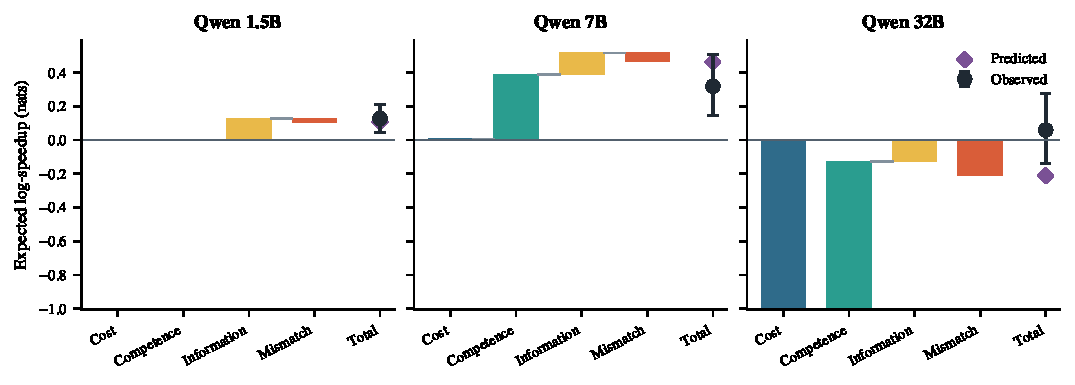
\includegraphics[width=0.92\textwidth]{figures/strategy_routing/four_term_accounting.pdf}
  \caption{\textbf{Diagnosing verified speed.}  Bars show per-step cost,
  competence, information, and mismatch; diamonds show the packed prediction
  and circles the observed packed log-speedup with task-bootstrap intervals.}
  \label{fig:four-term-accounting}
\end{figure*}

\subsection{Held-Out Allocation Test}

To isolate routing, we hold the worker model fixed.  Router model, context
length, and allocation head are chosen on the validation split subject to at
most one fewer verified success than the baseline.  Only the selected
configuration is then evaluated on the 42 untouched test tasks.

\begin{table}[t]
\centering
\small
\caption{Confirmatory paired test.  Speedup is the geometric mean of paired
solver-time ratios; intervals are 95\% task-bootstrap intervals.}
\label{tab:confirmatory-routing}
\begin{tabular}{@{}lccc@{}}
\toprule
Worker & Speedup & 95\% CI & Solved \\
\midrule
Qwen 1.5B & $0.951\times$ & $[0.855,1.060]$ & $34/42\to34/42$ \\
Qwen 7B   & $1.113\times$ & $[1.007,1.235]$ & $37/42\to37/42$ \\
Qwen 32B  & $0.855\times$ & $[0.742,0.961]$ & $36/42\to36/42$ \\
\bottomrule
\end{tabular}
\end{table}

At fixed 7B worker, the selected GPT-5.5 router with five in-context examples
and a performance-aware allocation head reduces arithmetic mean solver time
from $12.00$ to $9.54$ seconds while preserving all 37 verified successes.
The preregistered paired log metric gives the $1.113\times$ speedup in
Table~\ref{tab:confirmatory-routing}.  Router inference is excluded from this
solver-time comparison.  The batched router call took 102.5 seconds for 42
tasks, or 2.44 seconds per task under simple amortization; charging that amount
eliminates almost all of the arithmetic-mean end-to-end gain.

\begin{figure}[H]
  \centering
  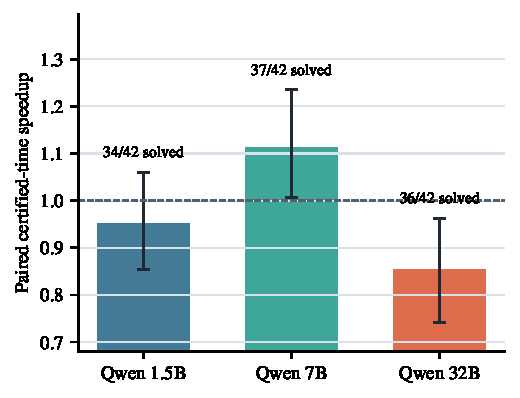
\includegraphics[width=\columnwidth]{figures/strategy_routing/confirmatory_speedup.pdf}
  \caption{\textbf{Held-out allocation speedup.}  Bars report paired
  solver-time speedup after validation-only configuration selection; error bars
  are 95\% task-bootstrap intervals.}
  \label{fig:confirmatory-speedup}
\end{figure}

\subsection{Estimators and Paired Validation}

For calibrated posteriors $\hat\pi_{Z_i}^M$ and realized allocations
$\hat q_i^M$, we estimate
\[
\hat G=H(\hat\pi)-\frac1N\sum_iH(\hat\pi_{Z_i}^M),
\qquad
\hat\varepsilon=\frac1N\sum_i
\KL(\hat\pi_{Z_i}^M\|\hat q_i^M),
\]
and estimate $\varphi$ from mode-conditioned packed scales.  Temperature
calibration and every allocation-head fit use only training or validation
records.  Task bootstrap preserves the paired comparison between baseline and
routed allocations.

\begin{proposition}[Paired allocation-gain estimator]
\label{prop:paired-unbiased}
Let $X_1,\ldots,X_N$ be i.i.d. deployment instances.  For condition
$k\in\{0,j\}$, let a fixed policy select action
$a_i^k=\rho_k(Z_k(X_i))$, where an action may be a retry allocation.  Let
$\ell(a,x;\xi)$ be an integrable deployment loss, and let
$\widehat m_j(x)$ be an unbiased estimate of the incremental signal cost
$m_j(x)$ in the same units as~$\ell$.  If each of $Q$ repeated runs has the
corresponding deployment distribution conditional on $(X_i,a_i^k)$, then
\begin{align*}
\overline\ell_i^k
&:=\frac1Q\sum_{q=1}^Q\ell(a_i^k,X_i;\xi_{i,q}^k),\\
\widehat\Delta_R(j)
&:=\frac1N\sum_{i=1}^N
\left[\overline\ell_i^0-\overline\ell_i^j-\widehat m_j(X_i)\right]
\end{align*}
is unbiased for the expected deployment gain net of signal cost.
\end{proposition}

\par\noindent\emph{Proof.} See Appendix~\ref{app:proof:paired-estimator}.\par
